% ______________________________________________________________________________
%
%   1DV607 Objectorienterad Analysis och Design med UML
%   Workshop 1 --- "Domain Modeling"
%
%  Author:  Jonas Sjöberg
%           Linnaeus University
%           js224eh@student.lnu.se
%           https://github.com/jonasjberg
%
% License:  Creative Commons Attribution 4.0 International (CC BY 4.0)
%           <http://creativecommons.org/licenses/by/4.0/legalcode>
%           See LICENSE.md for additional licensing information.
% ______________________________________________________________________________


% ______________________________________________________________________________
\section{Analysis}
The analysis is based on the given problem description\ref{probdesc}.
All work has been done by Jonas Sjöberg, without collaborators.


\subsection{Analysis of Requirements for Grade 2}
This analysis delimits the domain model to the following requirements:

\begin{itemize}
  \item \ref{usecase1} Authenticate
  \item \ref{usecase4} Register Boat
  \item \ref{usecase5} Remove Boat
  \item \ref{usecase6} Change Boat
  \item \ref{usecase8} Assign Berths
  \item \ref{usecase10} Manage Calendar Event
  \item \ref{usecase11} List Calendar Events
  \item \ref{usecase12} Show Calendar Event
\end{itemize}


\subsubsection{Domain Model for Grade 2}
\begin{figure}[htbp]
  \centering
  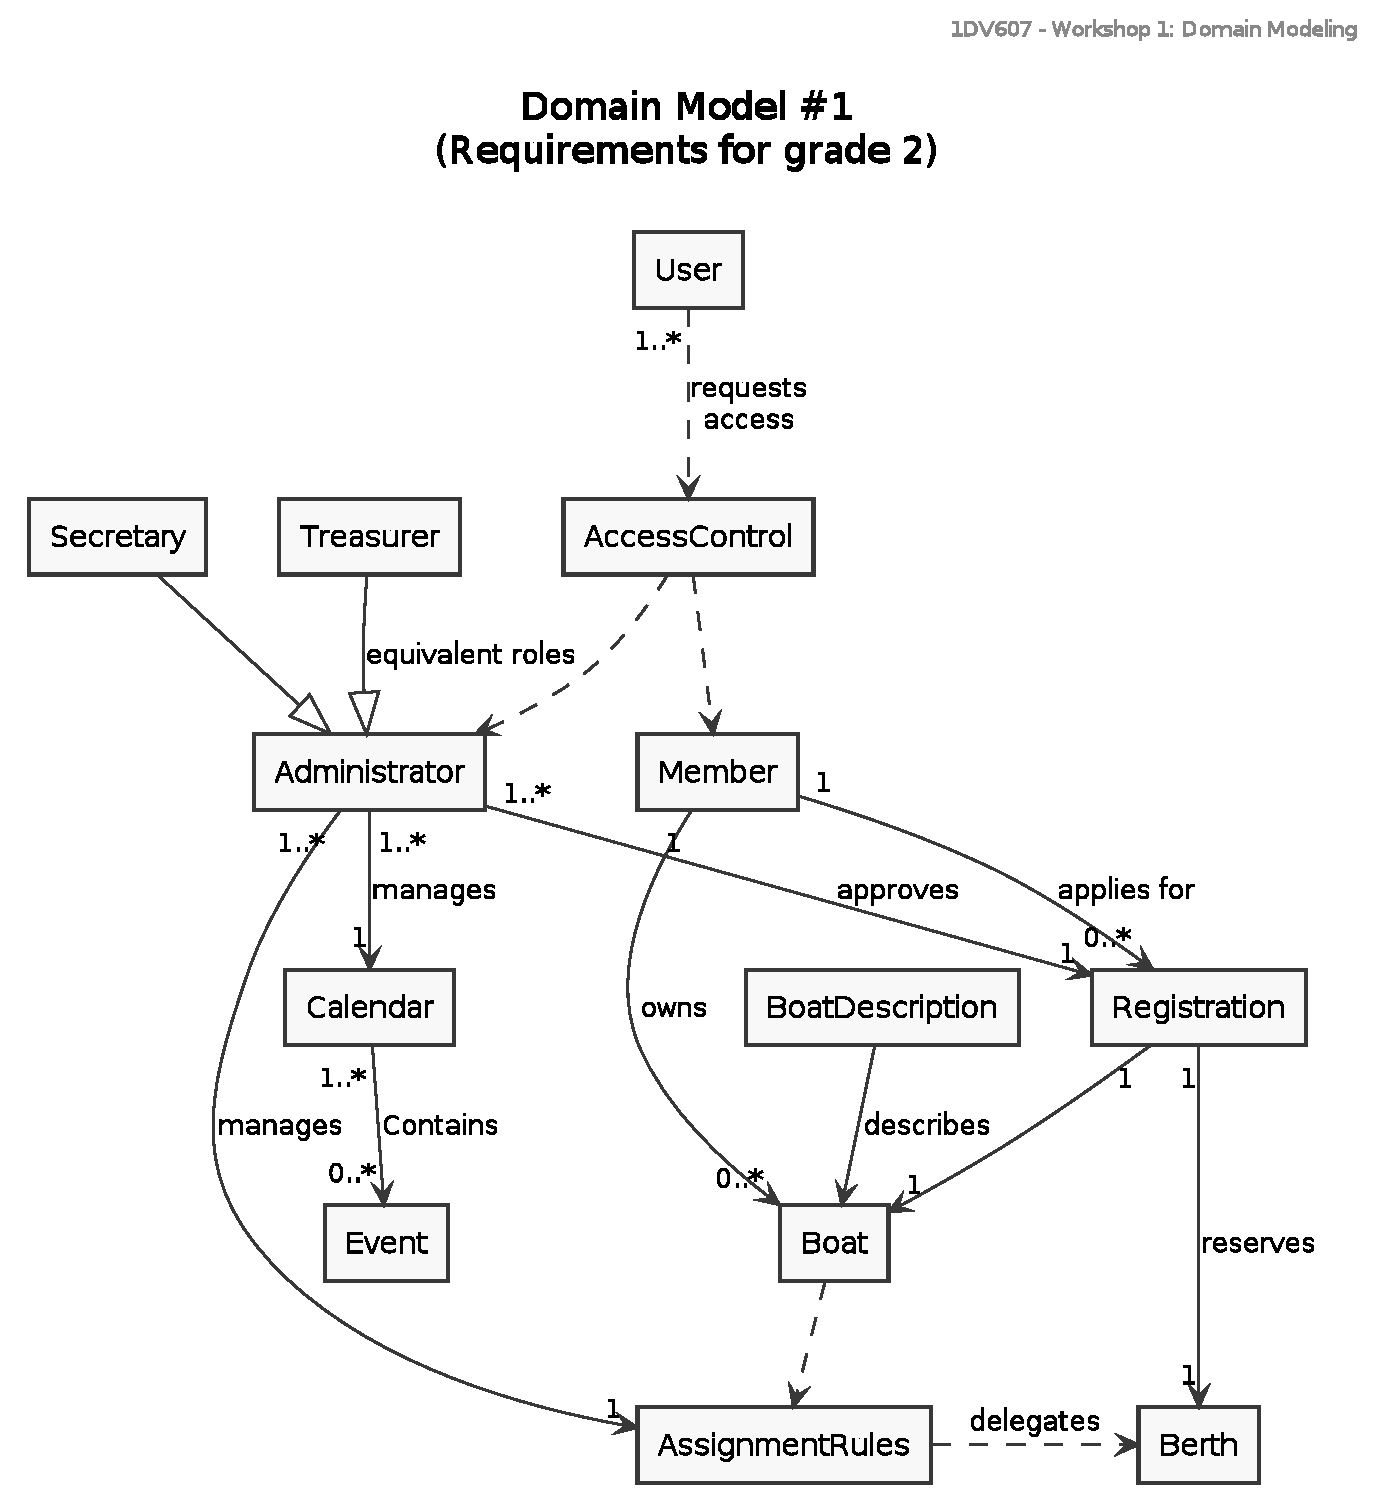
\includegraphics[width=\linewidth]{uml/domain-model_1.eps}
  \caption{UML Domain Model for Grade 2}
  \label{fig:uml-domain1}
\end{figure}

\subsubsection{Notes on the initial domain model}
The first domain model includes the concept of ``AccessControl'', just to
illustrate that the roles of ``Secretary'' and ``Treasurer'' are assumed to be
equivalent and are both treated as a form of ``Administrator''.

The administrators have elevated privileges, as compared to the ``Members''.



\subsection{Analysis of Requirements for Grade 3}
This analysis includes all of the requirements stated in the problem
description \ref{probdesc}.

\subsubsection{Domain Model for Grade 3}
\begin{figure}[htbp]
  \centering
  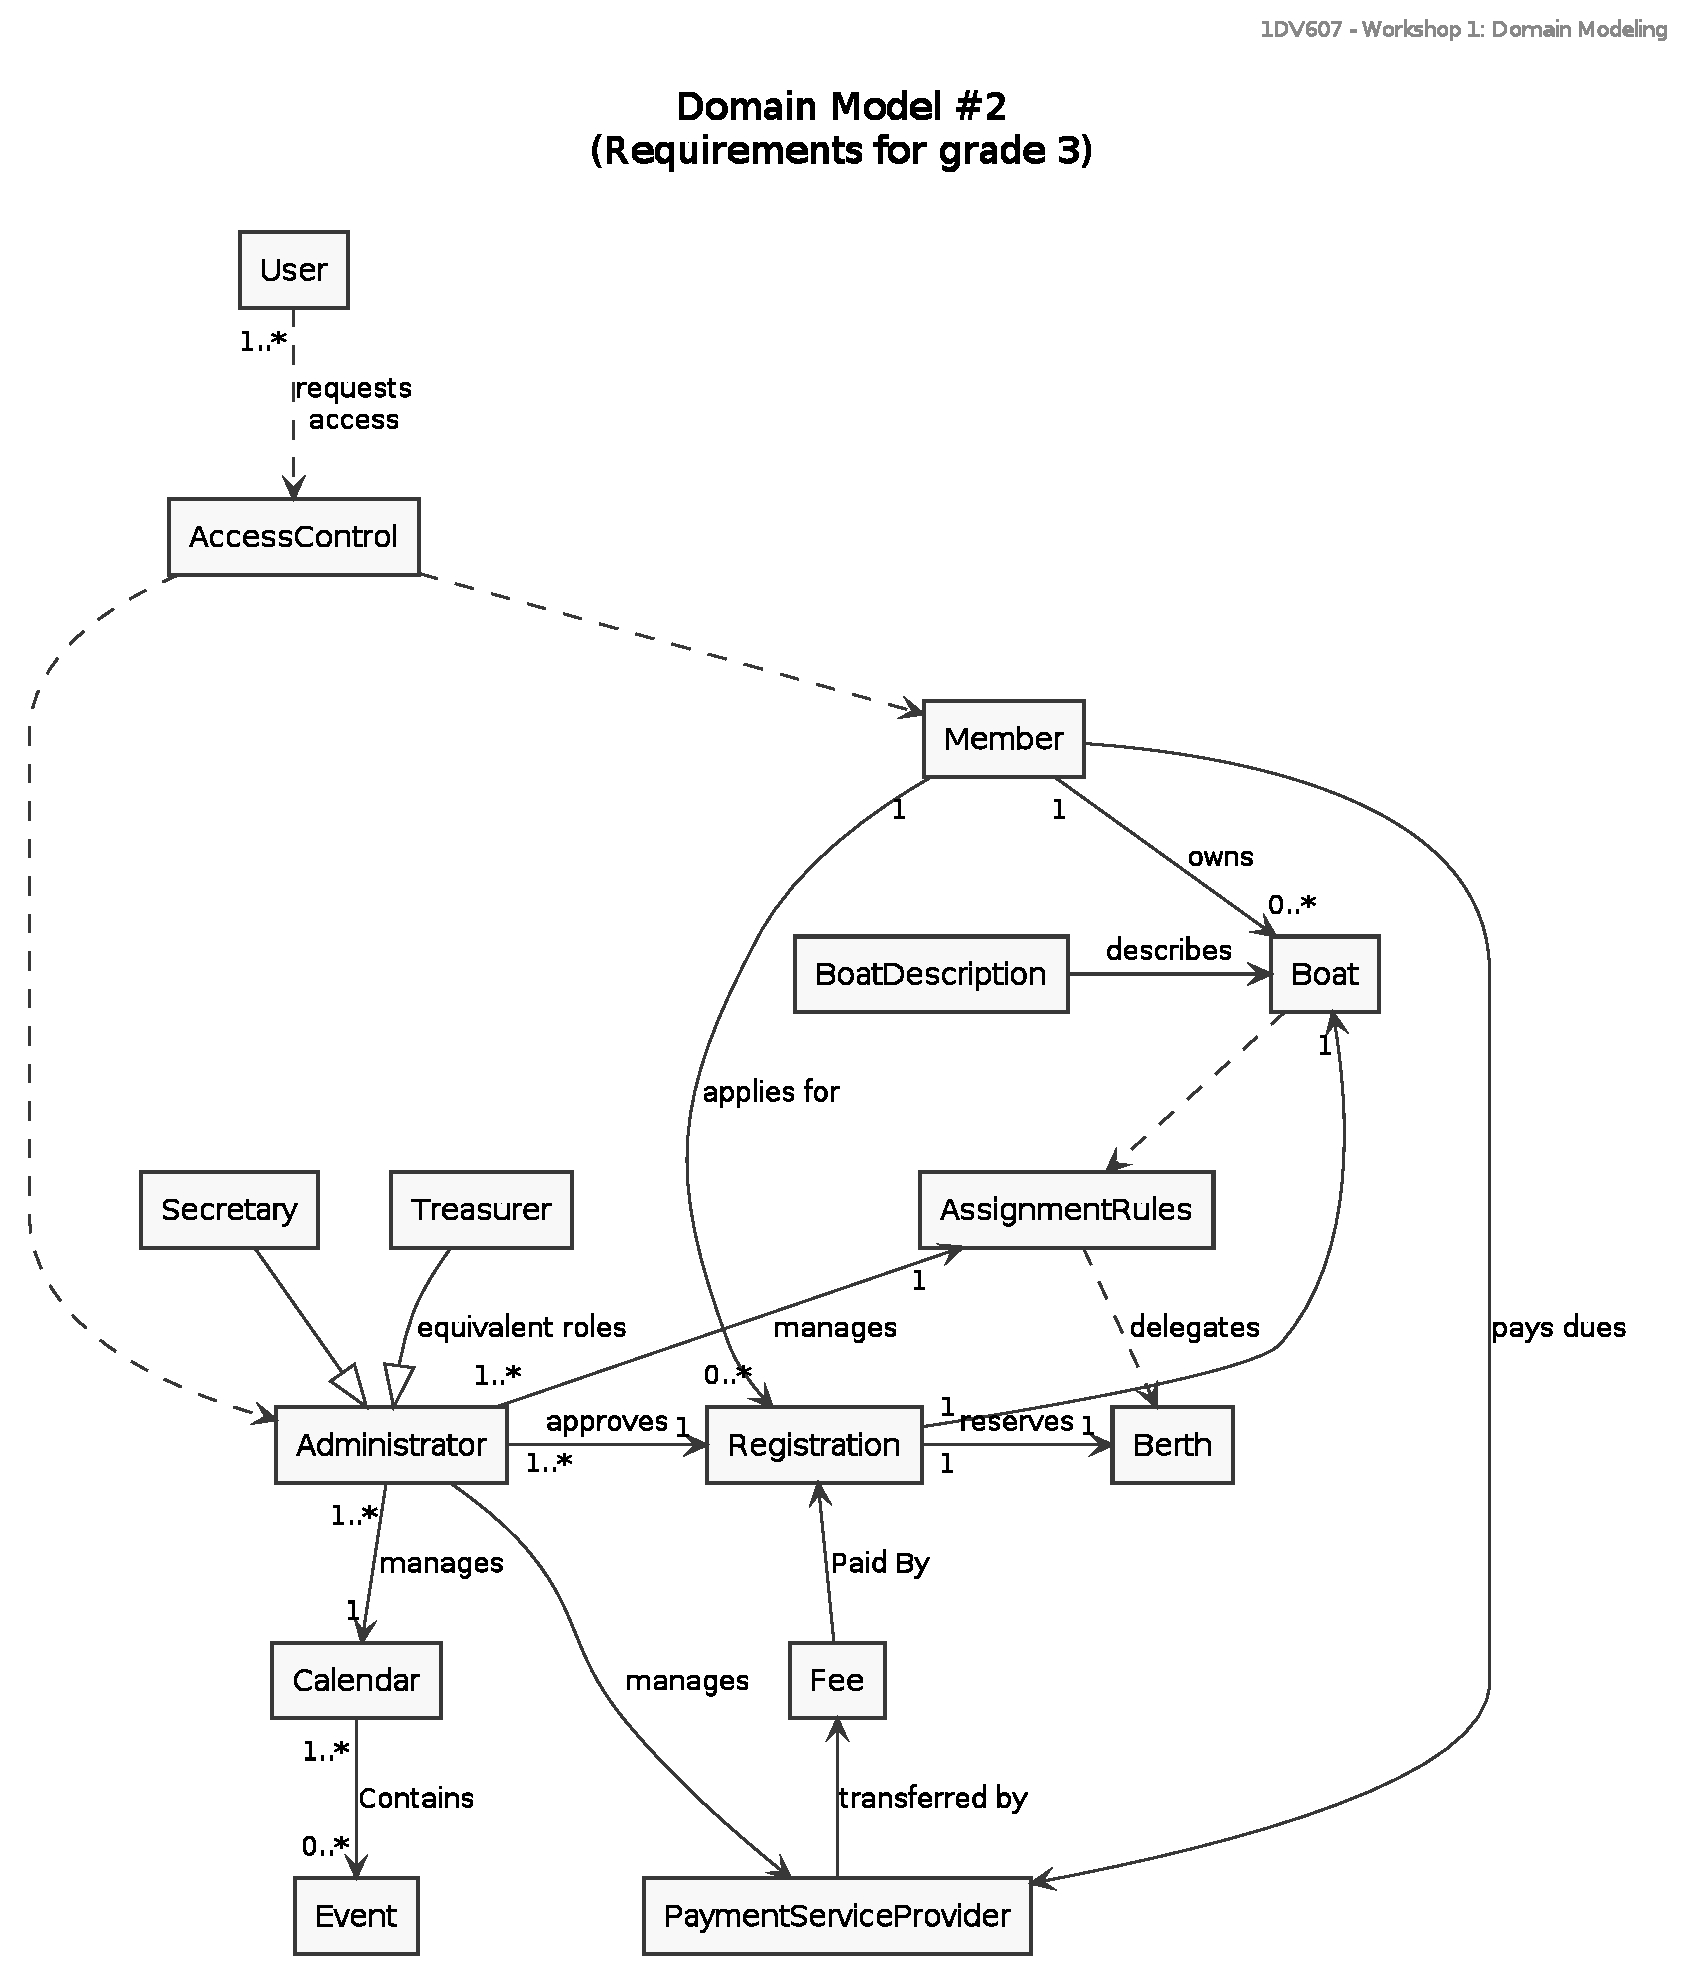
\includegraphics[width=\linewidth]{uml/domain-model_2.eps}
  \caption{UML Domain Model for Grade 3}
  \label{fig:uml-domain2}
\end{figure}

\subsubsection{Notes on the initial domain model}
The biggest change is the introduction of a payment service provider.

Most of the other requirements involve presentation of various data or managing
data in certain ways.  This is restricted to the different user-levels,
administrators should be able to manage invoices, etc.  These requirements
could be modeled with ``description classes'', which have been omitted for
clarity.


\subsection{Analysis of Requirements for Grade 4}
For this analysis, I've chosen to look at my open source project
``autonameow''\cite{js:autonameow-github}.  I've tried to model the system of
storage and retrieval of arbitrary data. However, this system is already
implemented and very complex --- the given model is incomplete and includes
many conflicting levels of abstraction.


\subsubsection{Notes on the main renaming actions in ``autonameow''}
The application collects as much data as possible from files. This includes the
file name, filesystem information, embedded metadata for various format,
textual contents, optical character recognition for images, etc. 

This data is then used to construct file names and rename files, using some
heuristics and user-control.

A highly simplified view of the main file remaing process is modeled in
Figure~\ref{fig:uml-domain3a}.


\subsubsection{Domain Model for Grade 3 -- file renaming in ``autonameow''}
\begin{figure}[htbp]
  \centering
  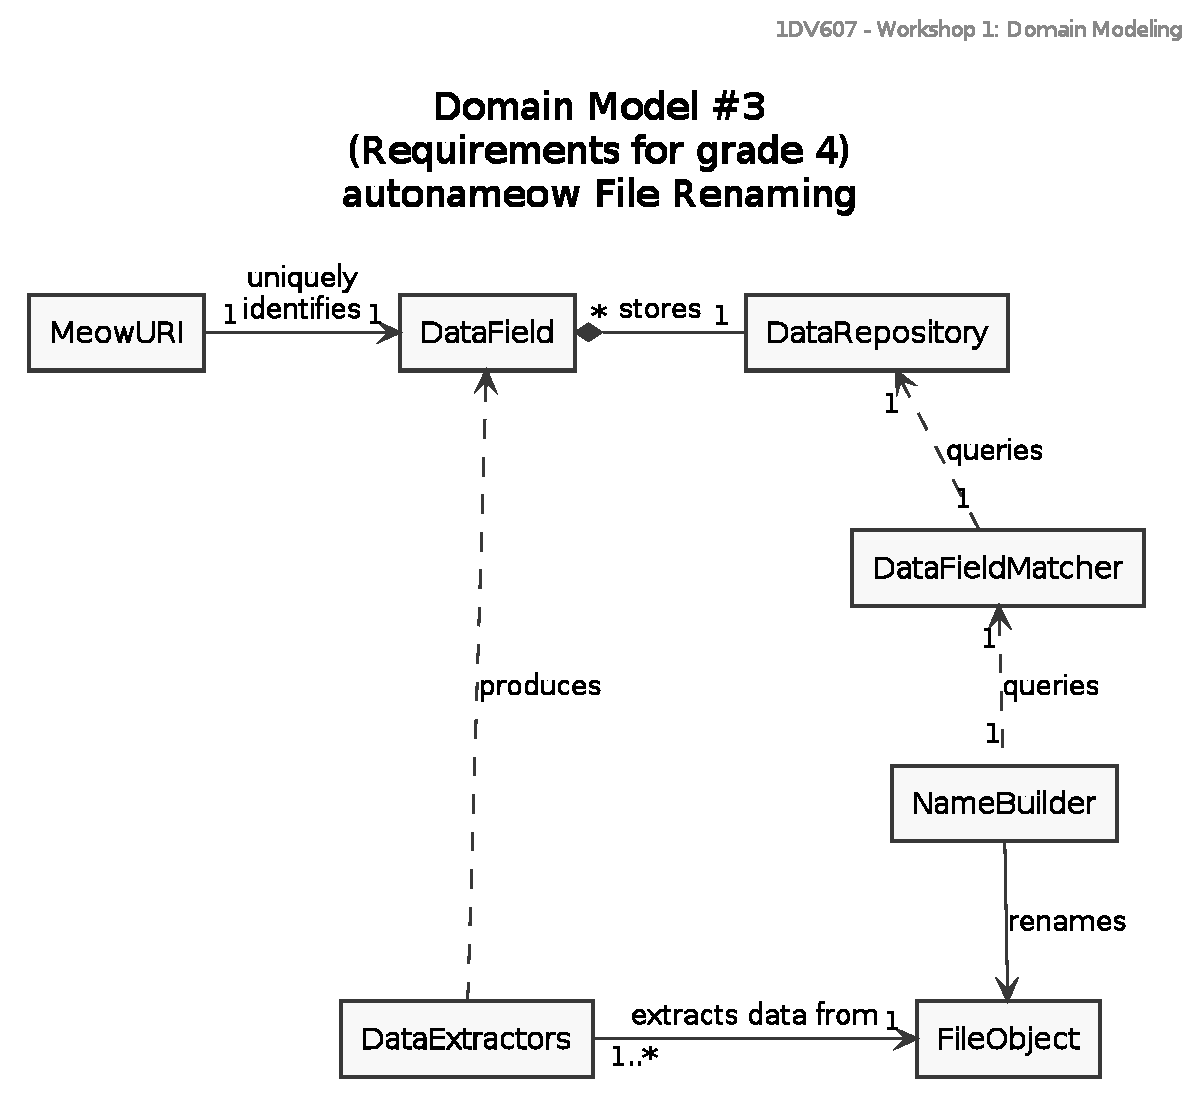
\includegraphics[width=\linewidth]{uml/domain-model_3a.eps}
  \caption{Domain Model of ``autonameow'' file renaming}
  \label{fig:uml-domain3a}
\end{figure}


\subsubsection{Notes on the ``autonameow'' data model}
Like a library or other storage system, stored data is given an identifier,
called a ``meowURI''; where ``URI'' is an abbreviation for Uniform Resource
Locator. These URIs provide the main means of querying and storing data.

A library might use ISBN- or EAN-numbers to identify specific items.
``autonameow'' also uses several identifiers, among these are ISBN-numbers,
which should be combined and weighted using some heuristics to produce a
suitable final result for any given query.
The user might want to include a creation date in the file name, the program
must then decide which of all the available date/time-information is most
likely ``correct''.


\subsubsection{Domain Model for Grade 3 -- data storage in ``autonameow''}
This model tries to capture the interaction between components. In practice, I
find that the interaction is too difficult to model properly at a level of
abstraction that would provide any additional insight, over what the source
code already provides.

A simplified model of the internal data storage is shown in
Figure~\ref{fig:uml-domain3b}.


\begin{figure}[htbp]
  \centering
  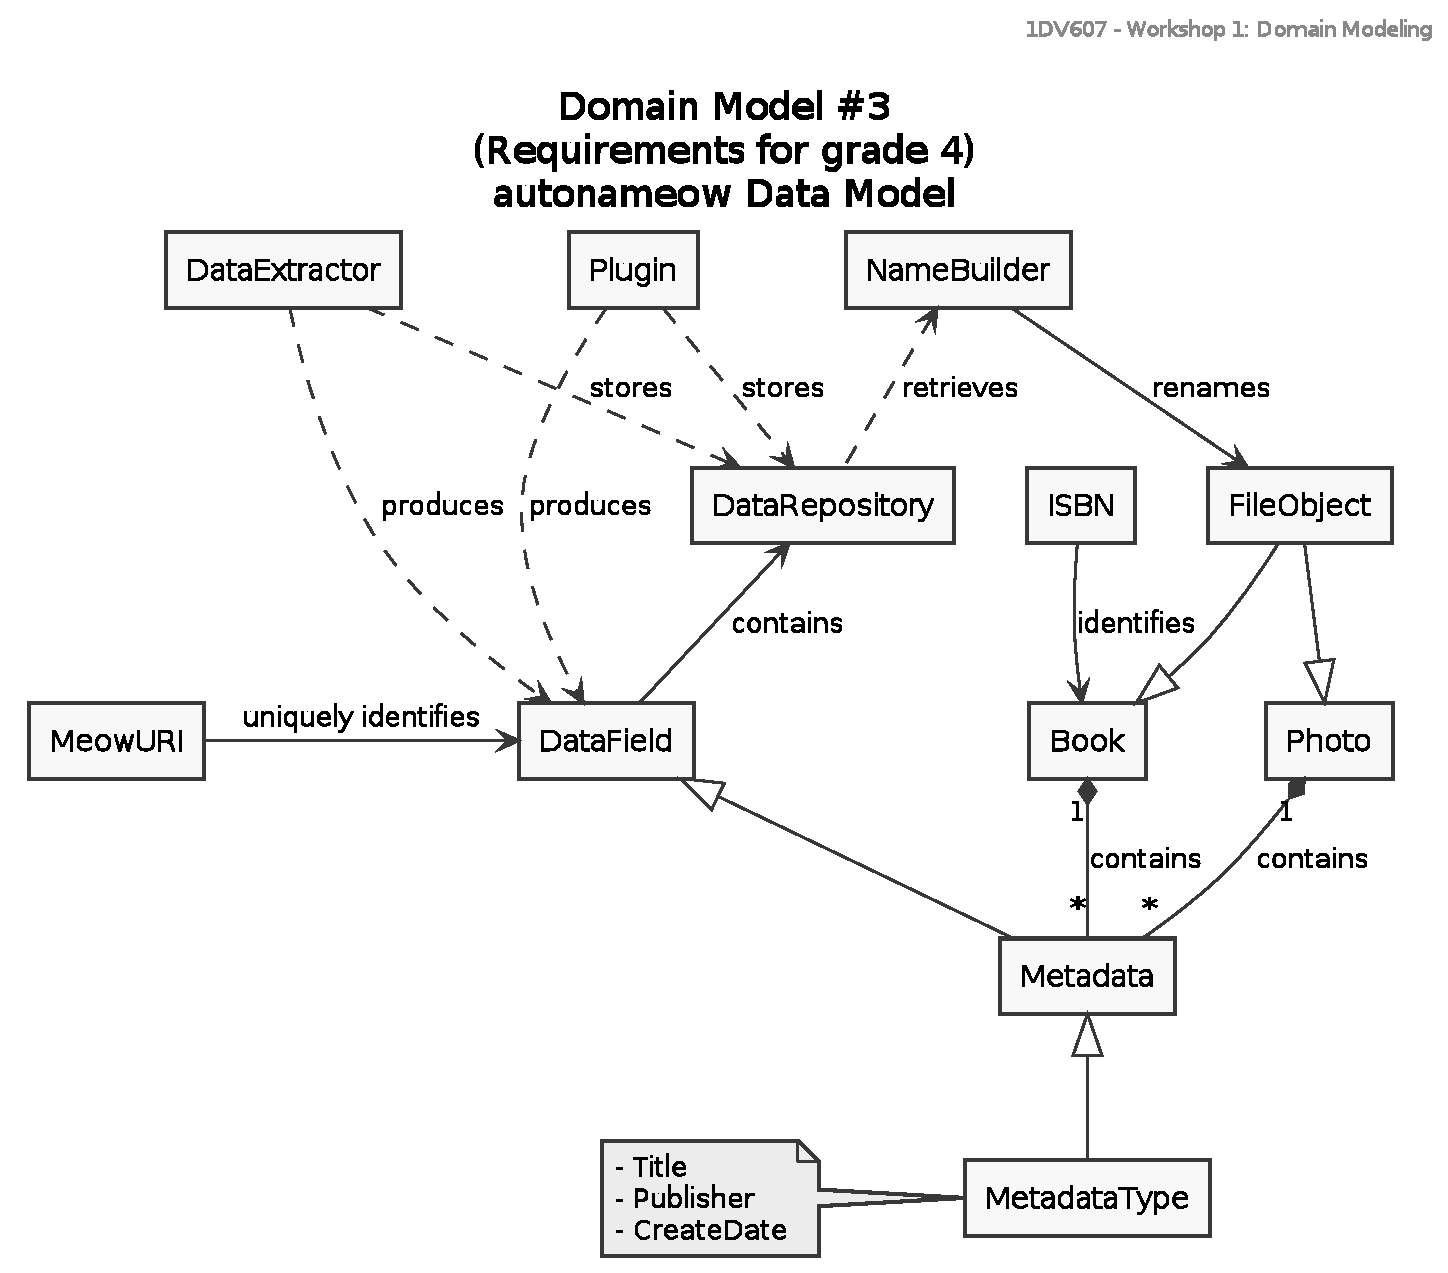
\includegraphics[width=\linewidth]{uml/domain-model_3b.eps}
  \caption{Domain Model of ``autonameow'' data storage}
  \label{fig:uml-domain3b}
\end{figure}

I've researched this topic for a very long time. A long list of references and
related projects or produces is included with the ``autonameow''
documentation\cite{js:autonameow-docs}.

Many models have proven incorrect or too complex. I will keep iterating and
redesigning the system until it meets the (ever changing) requirements.

I'm currently in the proces of redesigning the ``Repository'' to better handle
contextual information provided with a data item. Extracted metadata itself
often get additional metadata added on, containing the data source,
probabilities, primitive data types, etc \cite{metadata:aalemu-stevens}.
This has led me to research data repositories --- where methods of retrieval,
storage and presentation are all abstracted. I'm still reading up on how this
works.

